
% !TEX engine = latexmk -pdf
% !TEX buildOnSave = true
\documentclass[a4paper, 11pt, oneside]{article}

\usepackage[utf8]{inputenc}
\usepackage[T1]{fontenc}
\usepackage[french]{babel}
\usepackage{array}
\usepackage{shortvrb}
\usepackage{listings}
\usepackage[fleqn]{amsmath}
\usepackage{amsfonts}
\usepackage{fullpage}
\usepackage{enumerate}
\usepackage{graphicx}             % import, scale, and rotate graphics
\usepackage{subfigure}            % group figures
\usepackage{alltt}
\usepackage{url}
\usepackage{indentfirst}
\usepackage{eurosym}
\usepackage{listings}
\usepackage{color}
\usepackage[table,xcdraw,dvipsnames]{xcolor}

% Change le nom par défaut des listing
\renewcommand{\lstlistingname}{Extrait de Code}

\definecolor{mygray}{rgb}{0.5,0.5,0.5}
\newcommand{\coms}[1]{\textcolor{MidnightBlue}{#1}}

\lstset{
    language=C, % Utilisation du langage C
    commentstyle={\color{MidnightBlue}}, % Couleur des commentaires
    frame=single, % Entoure le code d'un joli cadre
    rulecolor=\color{black}, % Couleur de la ligne qui forme le cadre
    stringstyle=\color{RawSienna}, % Couleur des chaines de caractères
    numbers=left, % Ajoute une numérotation des lignes à gauche
    numbersep=5pt, % Distance entre les numérots de lignes et le code
    numberstyle=\tiny\color{mygray}, % Couleur des numéros de lignes
    basicstyle=\tt\footnotesize,
    tabsize=3, % Largeur des tabulations par défaut
    keywordstyle=\tt\bf\footnotesize\color{Sepia}, % Style des mots-clés
    extendedchars=true,
    captionpos=b, % sets the caption-position to bottom
    texcl=true, % Commentaires sur une ligne interprétés en Latex
    showstringspaces=false, % Ne montre pas les espace dans les chaines de caractères
    escapeinside={(>}{<)}, % Permet de mettre du latex entre des <( et )>.
    inputencoding=utf8,
    literate=
  {á}{{\'a}}1 {é}{{\'e}}1 {í}{{\'i}}1 {ó}{{\'o}}1 {ú}{{\'u}}1
  {Á}{{\'A}}1 {É}{{\'E}}1 {Í}{{\'I}}1 {Ó}{{\'O}}1 {Ú}{{\'U}}1
  {à}{{\`a}}1 {è}{{\`e}}1 {ì}{{\`i}}1 {ò}{{\`o}}1 {ù}{{\`u}}1
  {À}{{\`A}}1 {È}{{\`E}}1 {Ì}{{\`I}}1 {Ò}{{\`O}}1 {Ù}{{\`U}}1
  {ä}{{\"a}}1 {ë}{{\"e}}1 {ï}{{\"i}}1 {ö}{{\"o}}1 {ü}{{\"u}}1
  {Ä}{{\"A}}1 {Ë}{{\"E}}1 {Ï}{{\"I}}1 {Ö}{{\"O}}1 {Ü}{{\"U}}1
  {â}{{\^a}}1 {ê}{{\^e}}1 {î}{{\^i}}1 {ô}{{\^o}}1 {û}{{\^u}}1
  {Â}{{\^A}}1 {Ê}{{\^E}}1 {Î}{{\^I}}1 {Ô}{{\^O}}1 {Û}{{\^U}}1
  {œ}{{\oe}}1 {Œ}{{\OE}}1 {æ}{{\ae}}1 {Æ}{{\AE}}1 {ß}{{\ss}}1
  {ű}{{\H{u}}}1 {Ű}{{\H{U}}}1 {ő}{{\H{o}}}1 {Ő}{{\H{O}}}1
  {ç}{{\c c}}1 {Ç}{{\c C}}1 {ø}{{\o}}1 {å}{{\r a}}1 {Å}{{\r A}}1
  {€}{{\euro}}1 {£}{{\pounds}}1 {«}{{\guillemotleft}}1
  {»}{{\guillemotright}}1 {ñ}{{\~n}}1 {Ñ}{{\~N}}1 {¿}{{?`}}1
}
\newcommand{\tablemat}{~}

\definecolor{mymauve}{rgb}{0.58,0,0.82}

\begin{document}

\lstset{language=C, commentstyle={\color{blue}}, frame=single,
stringstyle=\color{magenta}}

\title{INFO0030: Projet 4}
\author{Groupe 33: Pavlov Aleksandr, Gendebien Alexandre}
\date{05.05.2025}

\maketitle
\section{Architecture générale de code}

Notre code est diviser en trois parties: le controller(controller), view(ui) et le model(Leaderboard,game).
De manière générale l'utilisateur interagit avec l'ui, qui elle-même interagit avec le controller,
qui gère les différentes fonctions d'interaction entre le model et l'ui(nottement les fonction qui demande d'afficher quelque chose à l'écran).

\section{Structures de données}

\textbf{Controller :}\\
Structure qui gère l’interaction entre le jeu et l’UI.

Coût en mémoire : faible (principalement des pointeurs et quelques variables).

\textbf{GameData :}\\
Contient tous les éléments essentiels au jeu : difficulté, taille de la grille, prochaines balles, le score et l'état du jeu (fini ou pas).

Pertinence : rassemble les informations du jeu pour un accès facile.

Coût en mémoire : dépend de la taille du champ de jeu et de la quantité de données stockées (dépend de la difficulté).

\textbf{Record :}\\
Garde en mémoire le nom du joueur et son score.

Pertinence : utile pour le classement général.

Coût en mémoire : faible, contient relativement peu d'informations.

\textbf{Leaderboard :}\\
Contient une liste triée des records, permettant l'affichage du classement des joueurs.

Pertinence : permet de conserver l'historique des scores et de les afficher.

Coût en mémoire : dépend du nombre de joueurs enregistrés, mais demande relativement peu de mémoire en général.

\textbf{Ui :}\\
Décrit l’UI avec divers éléments comme la fenêtre principale, la barre de menu, les boutons du jeu.

Pertinence : permet l'utilisation du système MVC.

Coût en mémoire : principalement des pointeurs vers des éléments GtkWidget, donc utilisation moyenne de la mémoire.

\section{Algorithmes particuliers}

\subsection{Calcul de la carte des distances (calculate\_distance\_map)}
Idée principale : Générer une carte des distances permettant de trouver la distance la plus courte entre `start` et `end`.

Pour trouver la distance la plus courte entre deux points, on a utilisé un algorithme du type **BFS** ou "Breadth-First Search".
L’algorithme BFS explore un graphe ou une grille en visitant tous les voisins d’une case avant de passer au niveau suivant.
Il fonctionne par expansion progressive, ce qui garantit qu’il trouve le chemin le plus court dans un environnement où chaque mouvement a le même coût.

\subsection{Calcul du chemin optimal (calculate\_path)}
Idée principale : Reconstruire le chemin optimal à partir de la carte des distances.

Parcours rétrograde à partir de `end`, en suivant les cellules ayant la plus petite distance séparant les deux points,
distance donnée par la fonction `calculate\_distance\_map`.
Puis retourne le chemin sous forme de tableau, facilitant le déplacement de la balle.

\subsection{Déplacement des balles}
Idée principale : Cette fonction gère le déplacement d'une balle d'une position `start` à une position `end` sur la grille.

À partir du chemin optimal entre les deux points (`start` et `end`), fourni par la fonction `calculate\_path`,
la balle est déplacée et l’état du jeu est mis à jour.

Puis met à jour la grille et place les prochaines balles si aucun alignement n'est détecté.

\section{Interface Graphique}

L’UI est composée d'une barre de menu contenant trois éléments : **Game, Difficulty et Help**.
\begin{itemize}
    \begin{figure}[h]
        \centering
        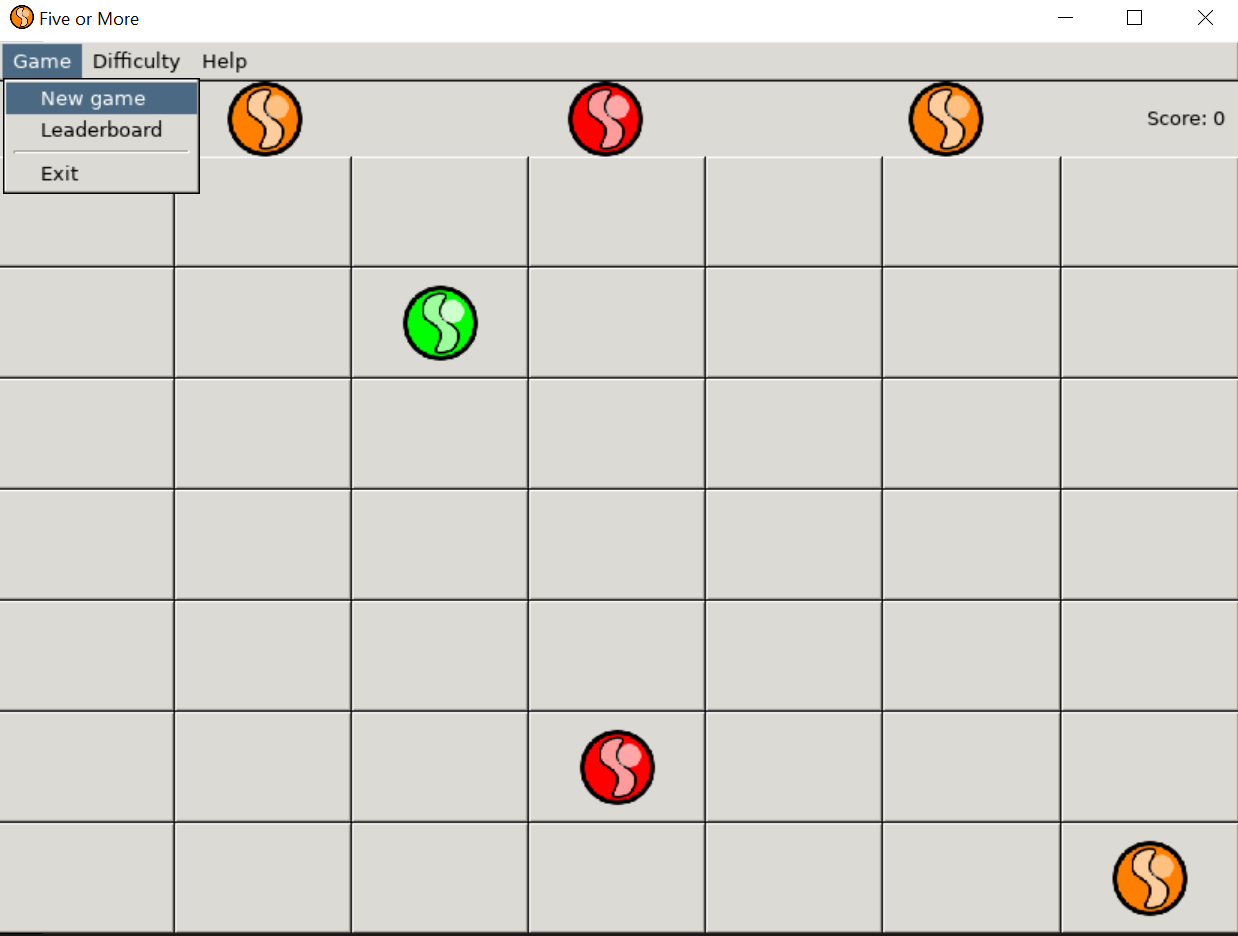
\includegraphics[width=0.7\textwidth]{menu.png}
        \caption{game menu}
    \end{figure}
    \item Le bouton \textbf{Game} contient un sous-menu à trois options : "New Game", "Leaderboard" et "Exit".
    \begin{figure}[h]
        \centering
        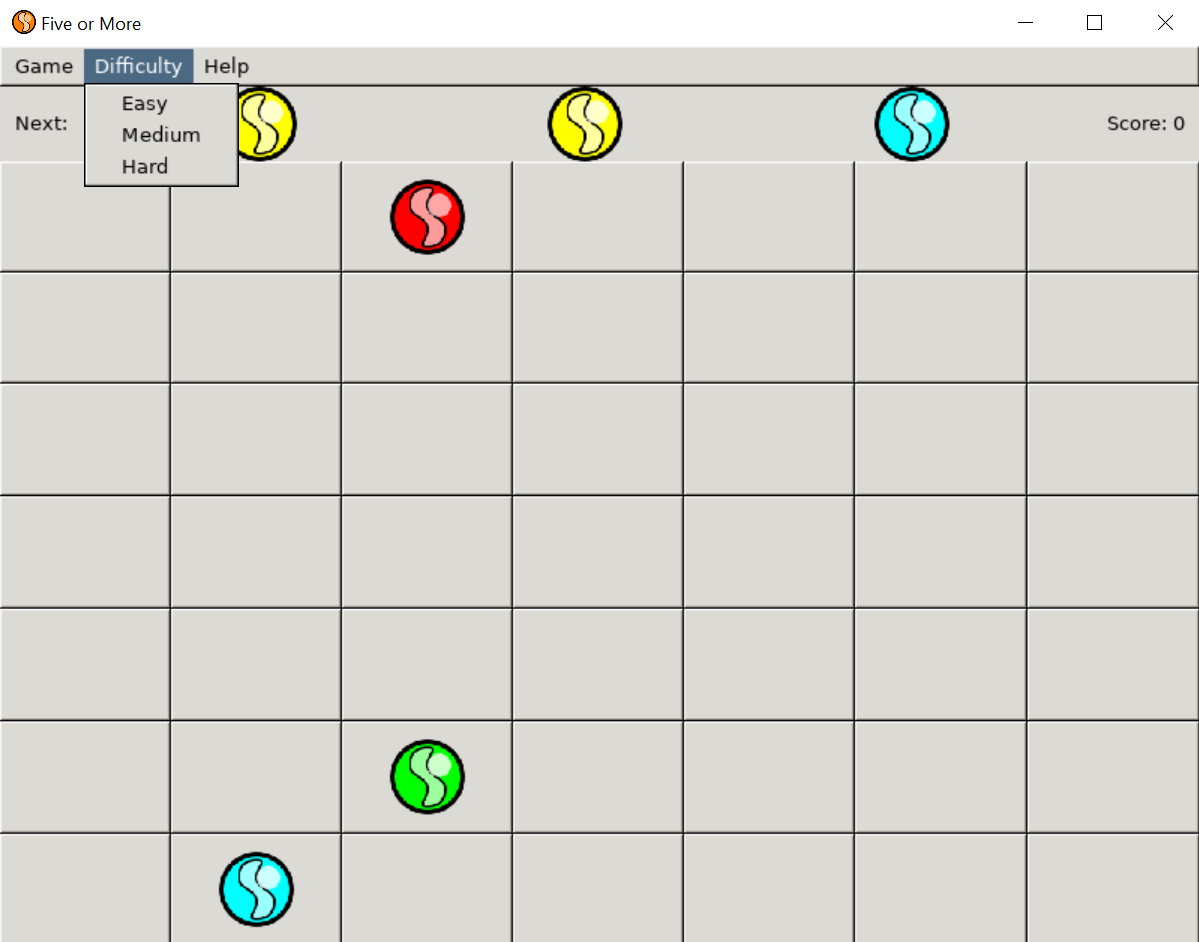
\includegraphics[width=0.7\textwidth]{difficulty.png}
        \caption{difficulty menu}
    \end{figure}
    \item Le deuxième élément de la barre de menu est un bouton qui contient un sous-menu avec les trois options : "Easy", "Medium" et "Hard".
    \begin{figure}[h]
        \centering
        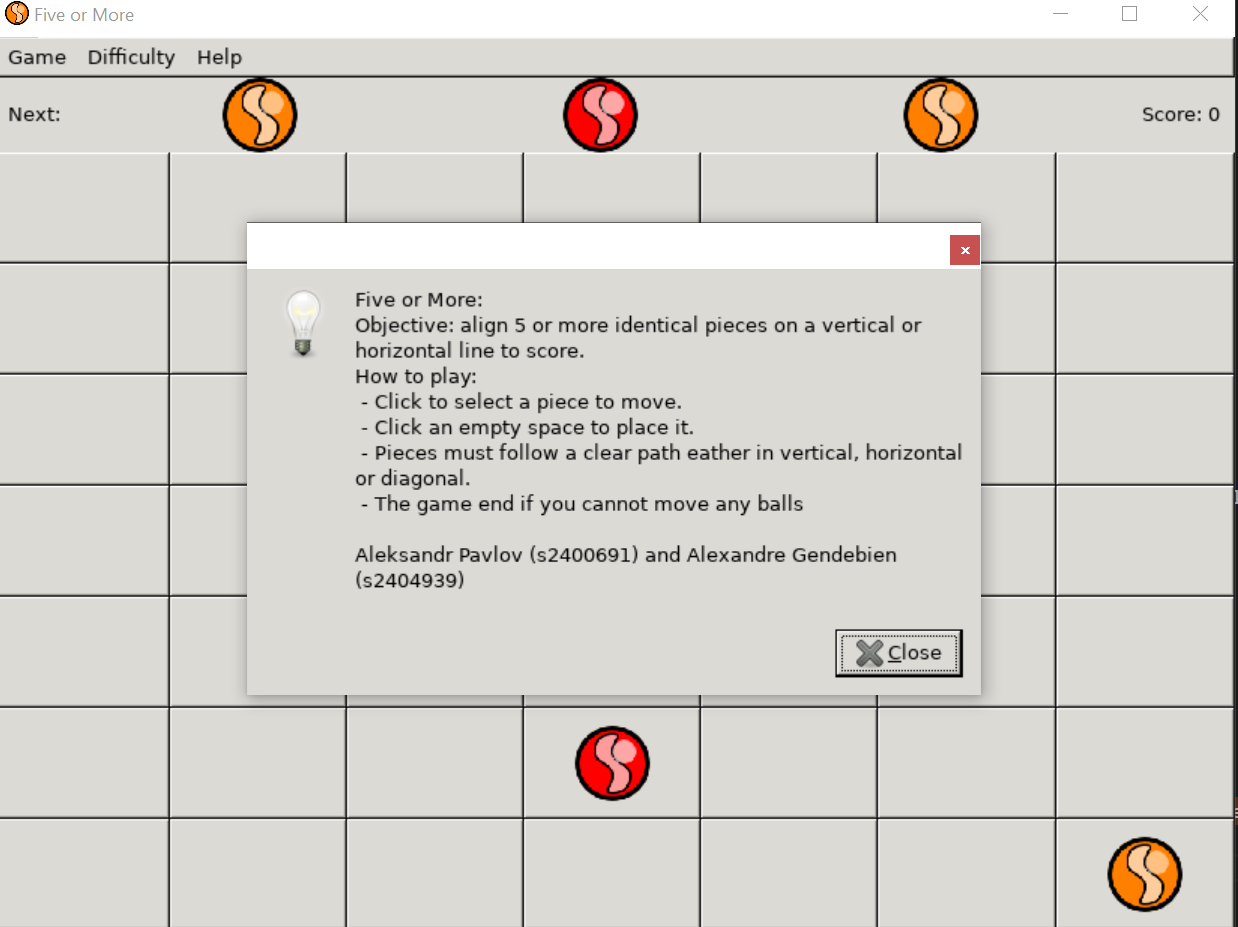
\includegraphics[width=0.7\textwidth]{help.png}
        \caption{help window}
    \end{figure}
    \item Le troisième élément de la barre de menu est le bouton "Help", qui affiche une fenêtre popup avec le guide d'utilisation du jeu ainsi que les règles de base.
\end{itemize}

La partie principale de l'UI est la \textbf{grille de jeu}, qui est composée de boutons stockés dans une **GtkVBox**, et les différentes `VBox` sont stockées dans une **GtkTable**.

C'est sur cette grille que se trouvent les éléments à déplacer (les balles). Entre la barre de menu et la grille :
\begin{itemize}
    \item Un \textbf{label} (à droite de l'écran) affichant le score actuel du joueur.
    \item Un affichage des \textbf{prochaines balles}, qui vont apparaître.
\end{itemize}

\section{Utilisation de GitLab pour la gestion du code}
On s’est principalement servi de Git pour partager les modifications que nous apportions au projet lors de son développement.
Un point positif que nous avons trouvé en utilisant la plateforme est que nous pouvions documenter nos modifications avant chaque envoi du code.
Cela nous a permis d’avancer plus vite, car il est plus facile de se partager le code de cette manière plutôt qu’autrement.
De plus, comme nous avons souvent un horaire de travail décalé l’un par rapport à l’autre, la documentation des commits nous permettait de rapidement nous remettre à jour par rapport à ce que l’autre avait fait pendant qu'il avançait sur le projet.

\section{Coopération dans le groupe}
Comme mentionné précédemment, Git a permis de grandement faciliter le travail et l’échange d’informations sur l’avancement du projet.
Mais pour résumer notre coopération : elle était basée sur une liste d’objectifs classés par ordre d’importance.
À chaque fois qu’un membre du groupe atteignait un certain quota d’objectifs, il envoyait le résultat sur Git, permettant ainsi au second membre d’avancer sur le projet et de prendre connaissance de ce qui avait été fait.

\section{Les améliorations possibles}
Comme c'est un jeu relativement basique, il n'y a pas énormément d'améliorations conséquentes que nous pourrions apporter à ce projet, à part :
\begin{itemize}
    \item Certaines améliorations graphiques.
    \item Le stockage des 10 meilleurs joueurs avec leurs scores sur un serveur, afin qu’il soit externe au programme et accessible à tous les utilisateurs.
\end{itemize}

\section{Nouveaux éléments appris}
Nous avons appris plusieurs choses durant le développement de ce projet, mais les deux plus importantes restent :
\begin{itemize}
    \item Comment faire une structuration efficace avec des modules indépendants (`ui`, `game`, `controller`…).
    \item Comment utiliser Git pour le suivi des versions et une collaboration plus efficace.
\end{itemize}

\end{document}
